\documentclass[10pt,a4paper]{amsart}
\usepackage[margin=19mm]{geometry}
\usepackage{amsmath,amssymb,mathtools}
\usepackage[scr=rsfs,cal=euler]{mathalfa}
\usepackage{xfrac}
\usepackage[unicode,hidelinks,bookmarks=false]{hyperref}
\newcommand{\ie}{i.e.\ }
\newcommand{\cf}{cf.\ }
\newcommand{\resp}{respectively\ }
\newcommand{\Subsection}{\subsection}
\providecommand{\nobreakdash}{\nobreak\hbox{-}}
\setlength{\emergencystretch}{2em}
\multlinegap0pt
\usepackage{tikz}
\usepackage{bm}
\usepackage{amssymb}
\usepackage{enumerate}
\newtheorem{theorem}{Theorem}
\def\graph{\mathrm{GRAPH}}
\title{Open Problems in Mathematical Logic}
\author{George Barmpalias, Su Gao, Jialiang He, Takayuki Kihara, Andre Nies, Theodore Slaman, Chieu-Minh Tran, Daniel Turetsky, Philip Welch, Liang Yu, Hang Zhang, George Barmpalias, Nikolay Bazhenov, Chi Tat Chong, Wei Dai, Su Gao, Jun Le Goh, Jialiang He, Keng Meng Selwyn Ng, Andre Nies, Theodore Slaman, Riley Thornton, Wei Wang, Jing Yu, Liang Yu}
\date{Source: arXiv:2608.26628v2 (CC BY 4.0)}
\begin{document}
\maketitle

\noindent\emph{Source and licence.} Open Problems in Mathematical Logic. Version arXiv:2608.26628v2 (CC BY 4.0), distributed by arXiv under the Creative Commons Attribution 4.0 International licence, http://creativecommons.org/licenses/by/4.0/, as recorded in the arXiv licence metadata for this exact version and shown on the abstract page https://arxiv.org/abs/2608.26628v2. Full licence notice: \texttt{licenses/arxiv-2608.26628-CC-BY-4.0.txt}.\par\smallskip

\noindent\textit{Editorial scope.} Counted unit: the article's theorem theorem (source0.tex lines 1891--1895). The article's complete original proof of it is delivered with it (source0.tex lines 1897--1924, one \texttt{proof} environment of 28 lines). No mathematics is written, repaired or re-derived: the statement and the proof are the article's own lines, in the article's own notation, and no retained line is substituted or re-flowed.  No further source-local context is needed: every cross-reference of every retained line resolves inside the two delivered spans.  Nothing was omitted from any retained span, so the package carries no omission record.  No retained line contains a citation, so the wrapper carries no bibliography and no bibliography entry.  The retained lines contain the article's own diagram code, which the wrapper typesets with the standard tikz packages; no image file is delivered and the package declares no asset dependency.  Editorial formatting only, in addition: an AMS \texttt{amsart} preamble that restates the article's own declarations and macros used by the retained lines, namely the environments \texttt{theorem} on separate counters, together with the standard packages those lines need.  The retained environments print in this document as Theorem 1 in order of appearance, whereas the article prints the same items with the numbering of its own full document.  The complete native source of the article as distributed in the arXiv e-print for this exact version is bundled unchanged as \texttt{sources/208650/source0.tex}.
\begin{theorem}[Feng Li--Ruiwen Li--Ming Xiao; Riley Thornton]
    The set
    $$\{G \in 2^{\omega \times \omega} : G \text{ is a graph on } \omega \text{ and } G \cong G^c\}$$
    is $\boldsymbol{\Sigma}_1^1$-complete.
\end{theorem}

\begin{proof}
    We define a continuous function $\Phi$ from $\graph^2$ to $\graph$, such that
    \begin{align*}
        (m,n) \in \Phi(G,H) \iff & m = 4k_1, n = 4k_2 \text{ and } (k_1,k_2) \in G; \\
        & m = 4k_1+1, n = 4k_2+1 \text{ and } (k_1,k_2) \in H^c; \\
        & m = 4k_1+2, n = 4k_2+2 \text{ and } (k_1,k_2) \in H^c; \\
        & m = 4k_1+3, n = 4k_2+3 \text{ and } (k_1,k_2) \in G; \\
        & m = 4k_1, n = 4k_2+1; \\
        & m = 4k_1+1, n = 4k_2+2; \\
        & m = 4k_1+2, n = 4k_2+3;
    \end{align*}

    The following figure depicts our definition for $\Phi$:
    \begin{figure}[htbp]
        \centering
        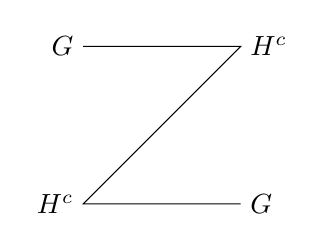
\begin{tikzpicture}
            \draw (0,0) node[left] {$G$} -- (2,0) node[right] {$H^c$} -- (0,-2) node[left] {$H^c$} -- (2,-2) node[right] {$G$};
        \end{tikzpicture}
    \end{figure}

    Now if $G \cong H$, it is easy to see $\Phi(G,H)$ is isomorphic to its complement.

    Conversely, if $\Phi(G,H) \cong \Phi(G,H)^c$, let $f$ be the witness of their isomorphism, and $d_1, d_2$ be the distance function on $\Phi(G,H)$ and $\Phi(G,H)^c$ respectively. Note that in $\Phi(G,H)$, $4\mathbb{N} \cup 4\mathbb{N}+3 = \{x \in \omega : \exists y \, d_1(x,y) = 3\}$. This is similar for $\Phi(G,H)^c$. So $f$ sends $4\mathbb{N} \cup 4\mathbb{N}+3$ to $4\mathbb{N}+1 \cup 4\mathbb{N}+2$. Also note that
    $$\{x \in \omega : \exists y \, (d_1(x,y) = 3) \land d_1(x,0) \leq 2\}$$
    is a copy of $G$,
    $$\{x \in \omega : \exists y \, (d_2(x,y) = 3) \land d_2(x,f(0)) \leq 2\}$$
    is a copy of $H$, and $f$ maps the former set to the latter set. So $G \cong H$.
\end{proof}

\end{document}
